\documentclass[12pt,letterpaper]{report}
\usepackage[utf8]{inputenc}
\usepackage[spanish]{babel}
\usepackage{amsmath}
\usepackage{amsfonts}
\usepackage{amssymb}
\usepackage{graphicx}
\usepackage[left=2cm,right=2cm,top=2cm,bottom=2cm]{geometry}
\author{Cruz Camacho Diego }
\title{operador jacoviano }
\begin{document}
\begin{center}
\emph{Operador Jacobiano}
\begin{flushleft}
En cálculo vectorial, se llama jacobiano o determinante jacobiano al determinante de la matriz jacobiana. Tanto la matriz jacobiana como el determinante jacobiano reciben su nombre en honor al matemático Carl Gustav Jacobi.
\begin{flushleft}
La matriz jacobiana es una matriz formada por las derivadas parciales de primer orden de una función. Una de las aplicaciones más interesantes de esta matriz es la posibilidad de aproximar linealmente a la función en un punto. En este sentido, el jacobiano representa la derivada de una función multivariable.Propiamente deberíamos hablar más que de matriz jacobiana, de diferencial jacobiana o aplicación lineal jacobiana ya que la forma de la matriz dependerá de la base o coordenadas elegidas. Es decir, dadas dos bases diferentes la aplicación lineal jacobiana tendrá componentes diferentes aún tratándose del mismo objeto matemático.
\begin{center}
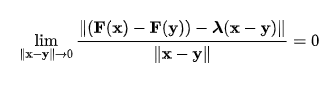
\includegraphics[scale=1]{1.PNG} 
\begin{flushleft}
\textbf{Función escalar}
\begin{flushleft}
Empecemos con el caso más sencillo de una función escalar {\displaystyle \scriptstyle F:\mathbb {R} ^{n}\to \mathbb {R} }\scriptstyle F:\mathbb{R} ^{n}\to \mathbb{R} .\\
 En este caso la matriz jacobiana será una matriz formada por un vector fila que coincide con el gradiente si la función admite derivadas parciales para cada variable puede verse que basta definir la "matriz" jacobiana como:
 \begin{center}
 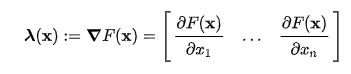
\includegraphics[scale=1]{2.PNG} 
 \begin{flushleft}
 \emph{Función vectorial}
 Supongamos {\displaystyle \mathbf {F} :\mathbb {R} ^{n}\to \mathbb {R} ^{m}}{\displaystyle \mathbf {F} :\mathbb {R} ^{n}\to \mathbb {R} ^{m}} \\
 Es una función que va del espacio euclídeo n-dimensional a otro espacio euclídeo m-dimensional. Esta función está determinada por m funciones escalares reales:
 \begin{center}
 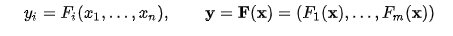
\includegraphics[scale=1]{3.PNG} 
 \begin{flushleft}
 Cuando la función anterior es diferenciable, entonces las derivadas parciales de estas m funciones pueden ser organizadas en una matriz m por n, la matriz jacobiana de F:
 \begin{center}
 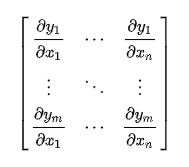
\includegraphics[scale=1]{4.PNG} 
 \begin{flushleft}
 Esta matriz es notada de diversas maneras:
 \begin{center}
 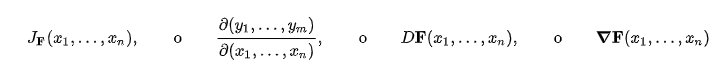
\includegraphics[scale=1]{5.PNG} 
 Nótese que la fila, i-ésima fila coincidirá dada con el gradiente de la función yi, para i = 1,...,m.

Si p es un punto de Rn y F es diferenciable en p, entonces su derivada está dada por JF(p). En este caso, la aplicación lineal descrita por JF(p) es la mejor aproximación lineal de F cerca del punto p, de esta manera:
\begin{center}
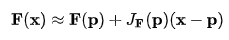
\includegraphics[scale=1]{6.PNG} 
\begin{flushleft}
\textbf{Invertibilidad y jacobiano}
\begin{flushleft}
Una propiedad interesante del jacobiano es que cuando éste es diferente de cero en el entorno de un punto dado, entonces el teorema de la función inversa garantiza que la función admite una función inversa alrededor de dicho punto.

El teorema anterior expresa una condición suficiente aunque no necesaria, ya que por ejemplo la función {\displaystyle \scriptstyle f(x)=x^{3}}\scriptstyle f(x)=x^{3}\\
 tiene por jacobiano {\displaystyle \scriptstyle J=3x^{2}}\scriptstyle J=3x^{2}\\
  que se anula en el punto {\displaystyle \scriptstyle x=0}\scriptstyle x=0,\\
  aunque alrededor de ese punto la función sigue teniendo inversa {\displaystyle \scriptstyle g(x)=f^{-1}(x)=x^{1/3}}\scriptstyle g(x)=f^{{-1}}(x)=x^{{1/3}}\\
   aun cuando el jacobiano es nulo en el origen.
\end{flushleft}
\end{flushleft}
\end{center}
 \end{center}
 \end{flushleft}
 \end{center}
 \end{flushleft}
 \end{center}
 \end{flushleft}
 \end{center}
\end{flushleft}
\end{flushleft}
\end{center}
\end{flushleft}
\end{flushleft}
\end{center}
\end{document}